\section{Yocto}
Depuis quelques années, avec l'arrivée de l'Internet Of Things (IOT), le monde de l'industrie se tourne davantage vers Yocto. Nous allons voir quels sont les avantages et inconvénients par rapport à Buildroot.
\subsection{La philosophie de Yocto}
Yocto est basé sur differents projets fusionnés en 2010. Supporté par les grands noms de l'industrie (Linux Fondation, Intel, AMD...), il porte un certain nombre d'évolutions :

\begin{itemize}
\item Gestionnaire de paquets (deb, ipk ou rpm)
\item Système de couches,chaque couche gérant un ensemble matériel ou logiciel. On peut retrouver ses couches \href{https://layers.openembedded.org}{\color{blue}Ici}. Elles sont directement utilisables par l'utilisateur.
\item Utilisation de bitbake, permettant de paralléliser et donc d'optimiser la compilation
\end{itemize}

Yocto permet de produire rapidement des distributions linux agiles, modulables et multi-platformes. Voyons ce que ces fonctionnalités permettent concretement.  

\subsection{Avantages}

\paragraph{}
Pour bien comprendre les avantages offerts par Yocto, prenons un exemple. On suppose ici que nous voulons construire une distribution avec un serveur graphique basé sur X11. Nous allons présenter de manière très synthétiques les étapes pour Buildroot et Yocto. 
\subsubsection{Configuration serveur graphique avec Buildroot}
\paragraph{}
Pour configurer un serveur graphique avec Buildroot, il vous faudra naviguer dans le menuconfig et sélectionner les bonnes options. Mais comment savoir lesquelles ? Il faut soit avoir une très bonne connaissance de X11 pour connaître tous les composants à activer, soit se référerer à un \href{https://agentoss.wordpress.com/2011/03/06/building-a-tiny-x-org-linux-system-using-buildroot/}{\color{blue}tutoriel} ou documentation. Dans le meilleur des cas, la configuration prendra une demi-heure, dans le pire une bonne journée. 

Si l'ajout de serveur graphique est à réaliser sur deux projets, il faudra refaire cette configuration pour les deux.

\subsubsection{Configuration serveur graphique avec Yocto}
\paragraph{}
Avec Yocto, l'installation est beaucoup plus simple. On tape 'x11' dans la \href{https://layers.openembedded.org/layerindex/branch/master/recipes/?q=x11}{\color{blue}base de donées des recettes}, on télécharge celle qui nous convient le mieux, et on l'ajoute avec la commande suivante : 

\$ bitbake-layers add-layer ??/meta-layer/

On compile et si le layer à été bien sélectionné, tout fonctionne. Dans le cas de deux projets, une même recettes convient aux deux. Si on la modifie elle le sera pour les deux.

\subsubsection{Des fonctionnalités bien pratiques}
C'est là l'énorme avantage de Yocto, une vaste communauté, avec des milliers de recettes existantes et maintenus à jour. Yocto permet donc de se focaliser sur le code métier, la vraie valeur ajoutée du produit développé et évite de devoir réinventer la roue à chaque fois. Le gestionnaire de paquets permet également de mettre à jours les différents composants via une simple commande, sans trop s'inquiéter des dépendances, et sans avoir besoin de recompiler l'image.



\paragraph{}
Le système de couche permet également une grande flexibilité en terme de fonctionnalités. Dans le cas d'une gamme de produit, avec une même base mais des options propres à chaque produit, l'utilisation des couches facilite le développement.

\begin{figure}[h!]
    \centering
    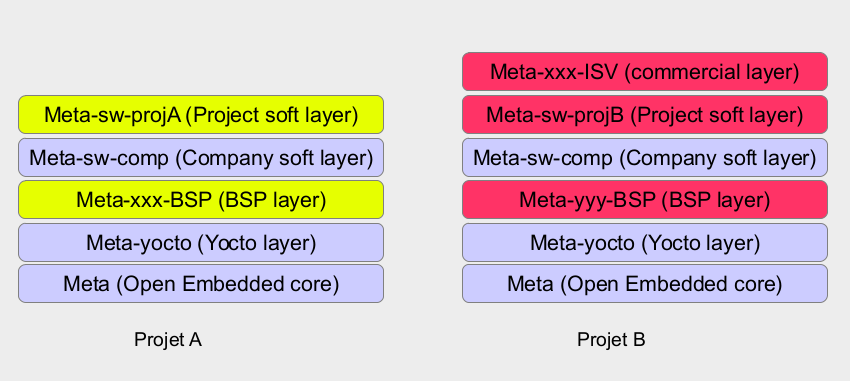
\includegraphics[width=10cm]{Images/reutilisable yocto.png}
    \caption{Système de couches permettant une factorisation. Credit : C. Charreyre}
\end{figure}